%%%%%%%%%%%%%%%%%%%%%%%%%%%%%%%%%%%%%%%%%%%%%%%%%%%%%%%%%%%%%%%%%%%%%%%%%%%%%%%%%%%%%%%%%%%%
%%
%% Chapter 3 : Related works
%%
%%      * Should give an overview of what the big dogs are saying in the field
%%
%%  BASIC STRUCTURE :
%%
%%      a. Current benchmarks for robot locomotion
%%          * DeepMind's controlsuite
%%          * OpenAI's mujoco-py
%%          * Berkeley's garage and rllab
%%          * Stanford's robosuite
%%          * UBC's terrainRlSim
%%          * Unity's ml-agents (talk about the marathon envs)
%%
%%      b. DRL algorithms for robot locomotion
%%          * Benchmarking drl in ccontrol environments (2016?)
%%          * Trust region policy optimization
%%          * Proximal policy optimization
%%          * DeepTerrainRL
%%          * DeepLoco
%%          * DeepMimic
%%          * Emergence of locomotion in rich and complex environments
%%
%%%%%%%%%%%%%%%%%%%%%%%%%%%%%%%%%%%%%%%%%%%%%%%%%%%%%%%%%%%%%%%%%%%%%%%%%%%%%%%%%%%%%%%%%%%%

\chapter{Related Works}
\label{ch:relatedWorks}

In this section we give an overview of the available RL benchmarks for continuous 
control, explaining each benchmark available, as well as a summary of the key characteristics
 of each one.

\section{DRL benchmarks for continuous control}

    \subsection{Control problems as early benchmarks}

    Some of the first benchmarks consisted of simple control problems, which included :

    \begin{itemize}
        \item \textbf{Inverted Pendulum}: make a simple 1 DOF actuated pendulum reach a vertical configuration.
        \item \textbf{Cart-pole}: make a non-actuated pendulum reach a vertical configuration by using an actuated horizontal base.
        \item \textbf{Mountain-car}: make a car reach a top position by means of swinging up and down a valley.
        \item \textbf{Acrobot}: make a double pendulum reach a vertical configuration by means of only the second actuated joint.
    \end{itemize}

    These early benchmarks were low dimensional \textbf{continuous} state and actions spaces, 
    and most of them consisted of symbolic forms with no "simulation" (implementing and simulating
    the exact model using the modeled dynamics of the task). 

    \subsection{Simulated environments}
    
    More recently simulated environments started to be used, which built on top of current 2D and 3D
    physics engines. These allowed to easily configurate new tasks, and also allowed to use tasks 
    with more complicated dynamics. We will focus on these as they are the basis for the current
    available benchmarks for continuous control. The basic structure of these benchmarks is shown in Figure 2.1, and consists of :

    \begin{itemize}
        \item \textbf{Physics Engine} : The engine used for physics simulation. Available choices are Box2D \citep{Box2D},
                Bullet \citep{Bullet}, DART \citep{DART} and MuJoCo \citep{MuJoCo}.
        \item \textbf{RL interface} : This is the software interface between the user and the physics engine itself. The 
                benchmarks usually expose an API for initialization and interaction with the simulated agent, as well as 
                some other functionality for the user that returns the necessary components to train a RL agent (like observations,
                state, action space, etc.). Some examples of these interfaces include Controlsuite \citep{Controlsuite}, 
                OpenAI-Gym \citep{Gym}, rllab \citep{Rllab}, garage \citep{garage} and unity ml-agents \citep{unity-ml-agents}.
        \item \textbf{User code} : This is usually left for the user. Some benchmarks are part of a framework, which gives the user
                a starting interface to implement the required RL algorithm. Some others don't include this layer of abstraction, and
                leave the user in charge of implementing the RL agent based on the exposed API from the RL interface.
    \end{itemize}

    \begin{figure}[!ht]
	\centering
	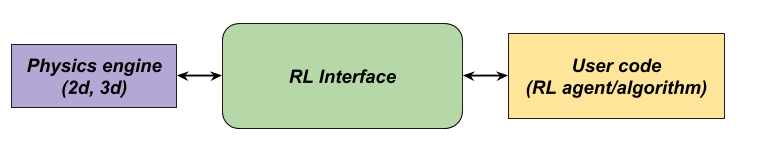
\includegraphics[width=4.5in]{./chapters/imgs/img_base_sim_env.png}
	\caption[Basic structure of a simulated environment]{Base architecture of simulated environments}
	\label{fig:sim-env}
    \end{figure}

\section{Current available benchmarks}

    In this section we will explain in a bit more detail the current benchmarks used for DRL research in
    continuous control tasks. These are based on the previously mentioned architecture, and vary depending 
    of the way each of the three main components are built.

    \subsection{Deepmind Control Suite}
    This suite of benchmarks consists of a Python wrapper of the MuJoCo physics engine, and a RL API on top
    exposed to the user for the creation of the RL agent. This suite is separated in \textbf{models} and \textbf{tasks},
    being a task an instance of a specific model (like humanoid, cartpole, etc.), and a task being the setup that
    the agent must solve, e.g. stand, walk, or run in the case of the humanoid model.
    \\
    \\
    As the author explain in its technical report \citep{Controlsuite}, they built a standarized RL API with 
    the following features :

    \begin{itemize}
        \item \textbf{Full observations}: the agent receives the full state as observation.
        \item \textbf{Normalized actions}: the actions exposed to the user are in the range $\left[-1,1\right]$.
        \item \textbf{Normalized rewards}: the rewards are set to the range $\left[ 0, 1 \right]$, and can be smooth (whole range)
                or sparse (just the values $\left\{0,1\right\}$).
    \end{itemize}

    Below we show a figure from the environments presented by this benchmark.

    \begin{figure}[!ht]
        \centering
        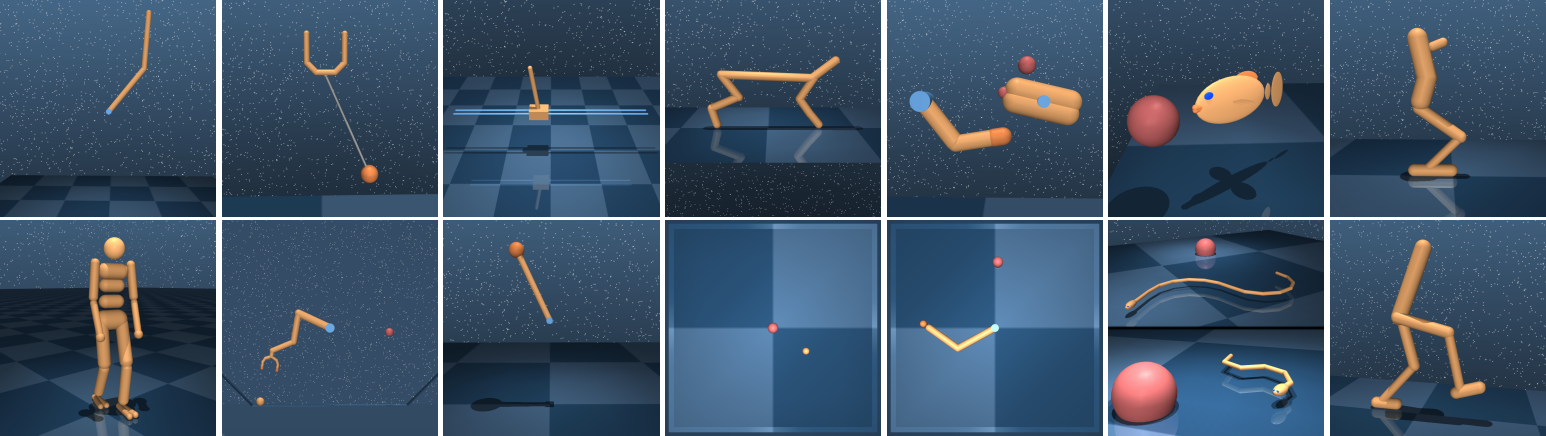
\includegraphics[width=5.5in]{./chapters/imgs/img_controlsuite_envs.png}
        \caption[Controlsuite models]{Models available in the Controlsuite benchmark. Extracted from \citet{Controlsuite}.
                                      Models from the BENCHMARK set of environments.}
        \label{fig:controlsuite-envs}
    \end{figure}

    \subsection{OpenAI Gym}
    This set of benchmarks consists of two separate options, depending on the physics engine to be used. These options are :

    \begin{itemize}
        \item \textbf{Mujoco-py} : A Python wrapper for MuJoCo, very similar to Controlsuite. The tasks it
            exposes are also similar to the ones in Controlsuite, which are shown in figure 2.3 . This acts as
            the physics backend to be used for the RL API defined by Gym itself.
        \item \textbf{RoboSchool}: An implementation that uses PyBullet, which are bindings for the Bullet physics
            engine. The environments exposed are a bit different to the previous suite, and are shown in figure 2.4 . It
            also serves as a physics backend for the Gym RL API.
    \end{itemize}

    \begin{figure}[!ht]
        \centering
        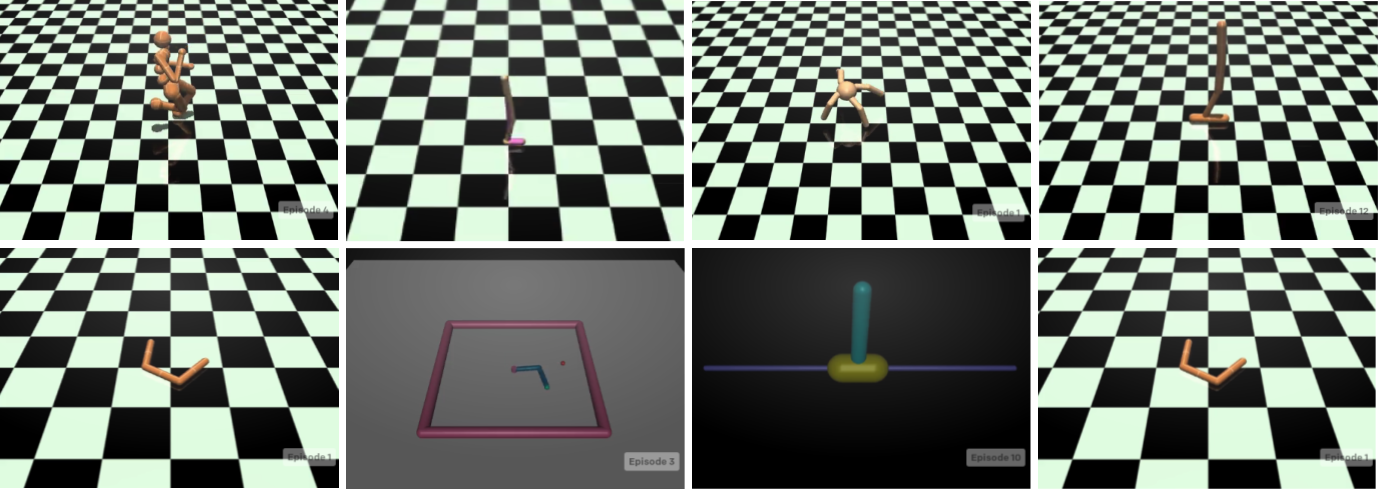
\includegraphics[width=5.5in]{./chapters/imgs/img_openai_gym_mujoco_envs.png}
        \caption[Gym Mujoco models]{Models available in the Gym-Mujoco benchmark. Extracted from \citet{OpenAIgym}}
        \label{fig:gym-mujoco-envs}
    \end{figure}

    \begin{figure}[!ht]
        \centering
        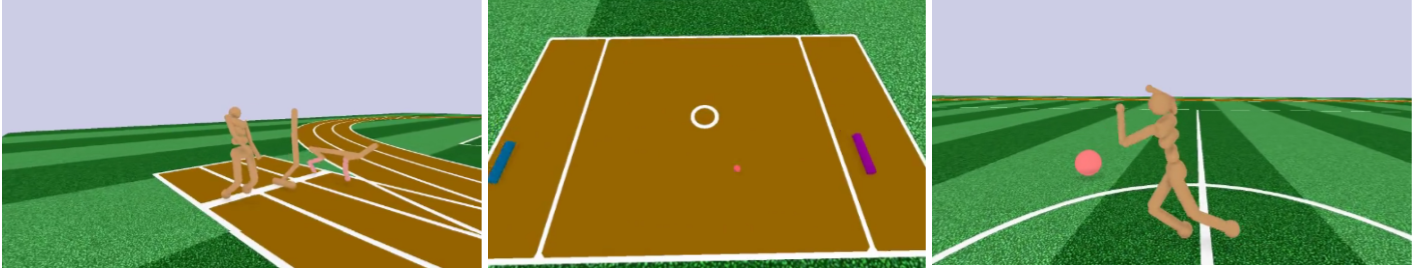
\includegraphics[width=6.0in,height=2.0in]{./chapters/imgs/img_openai_gym_roboschool_envs.png}
        \caption[Gym RoboSchool models]{Models available in the Gym-RoboSchool benchmark. Extracted from \citet{OpenAIgym}}
        \label{fig:gym-roboschool-envs}
    \end{figure}

    The RL API exposed by Gym is similar to the one exposed by Controlsuite. In each step taken in the environment, the API
    returns the observation, reward, and some extra information. The user selects which More can be found in its technical report \citep{OpenAIgym}, and
    in its repository at \url{https://github.com/openai/gym}.

    \subsection{Rllab}
    This set of benchmarks is quite similar to the previous two. It implements its own Python wrapper for MuJoCo, and 
    builds its own RL API on top of that wrapper. This suite is a bit different to the other two, because it provides
    a set of tested baselines of various DRL algorithms, which were compared in \cite{Rllab}. The environments provided 
    by rllab are grouped in three categories: \textbf{classic} (figure 2.5), \textbf{locomotion} (figure 2.6) and 
    \textbf{hierarchical} (figure 2.7).

    It is compatible with Gym, by means of a wrapper on top of its environments, but as they explain in their documentation
    website (\url{https://rllab.readthedocs.io/en/latest/user/gym_integration.html#}) this is a very different API.

    \begin{figure}[!ht]
        \centering
        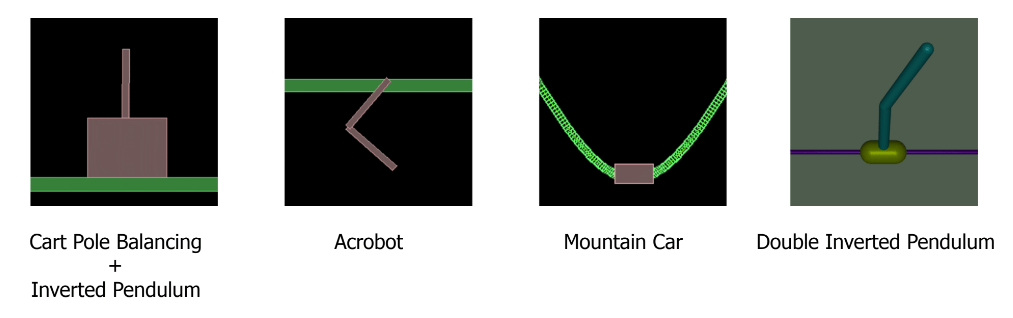
\includegraphics[width=5.0in]{./chapters/imgs/img_rllab_envs_classic.png}
        \caption[rllab classic models]{Models available in the Rllab classic benchmark. Extracted from \citet{Rllab}}
        \label{fig:rllab-envs-classic}
    \end{figure}

    \begin{figure}[!ht]
        \centering
        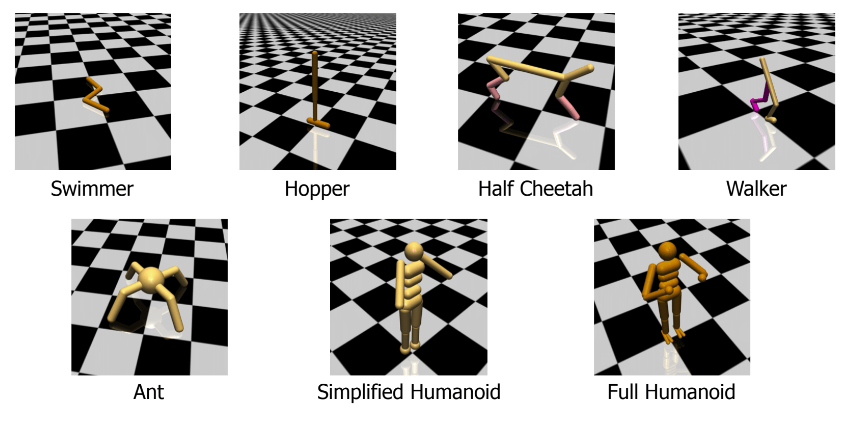
\includegraphics[width=4.5in]{./chapters/imgs/img_rllab_envs_locomotion.png}
        \caption[rllab locomotion models]{Models available in the Rllab locomotion benchmark. Extracted from \citet{Rllab}}
        \label{fig:rllab-envs-locomotion}
    \end{figure}

    \begin{figure}[!ht]
        \centering
        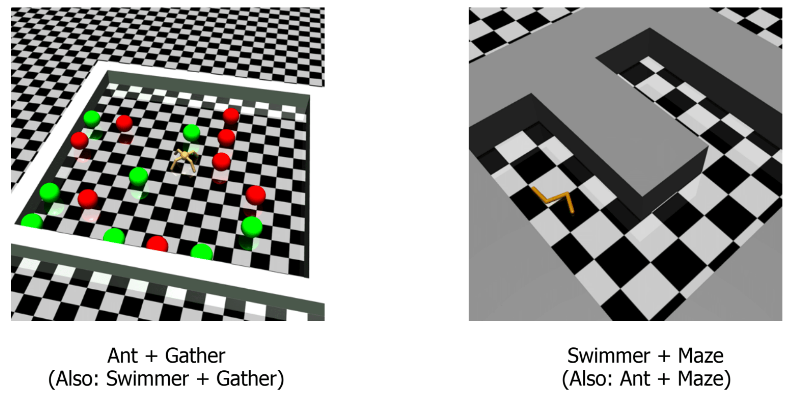
\includegraphics[width=5.0in]{./chapters/imgs/img_rllab_envs_hierarchical.png}
        \caption[rllab hierarchical models]{Models available in the Rllab hierarchical benchmark. Extracted from \citet{Rllab}}
        \label{fig:rllab-envs-hierarchical}
    \end{figure}

    \subsection{Garage}
    Garage is the next version of the rllab suite, and is very similar in architecture to the rllab suite, with support
    for more environments and baselines. To this date the number of environments is similar to the ones in rllab, but is
    being actively supported, compared to the rllab. More information can be found in its repo (\url{https://github.com/rlworkgroup/garage}).
 
    \subsection{Unity ML-Agents}
    This last suite \citep{unity-ml-agents} is a recent one, and consists of some ports of the previously mentioned environments, as well
    as many more new environments that are built on top of the \citeauthor{unity} game engine. These allows to easily create new environments
    for RL agents because of all the tools provided by the Unity3d engine.

    One of the key differences is the type of physics engine used, which in this case is the \citeauthor{physX} (a real time physics engine
    developed by NVIDIA for games). Compared with MuJoCo, this is less optimized for multibody dynamics. Instead, it is optimized to simulate
    lots of objects. Another key difference is the RL API, which has the architecture shown in figure 2.8.

    \begin{figure}[!ht]
        \centering
        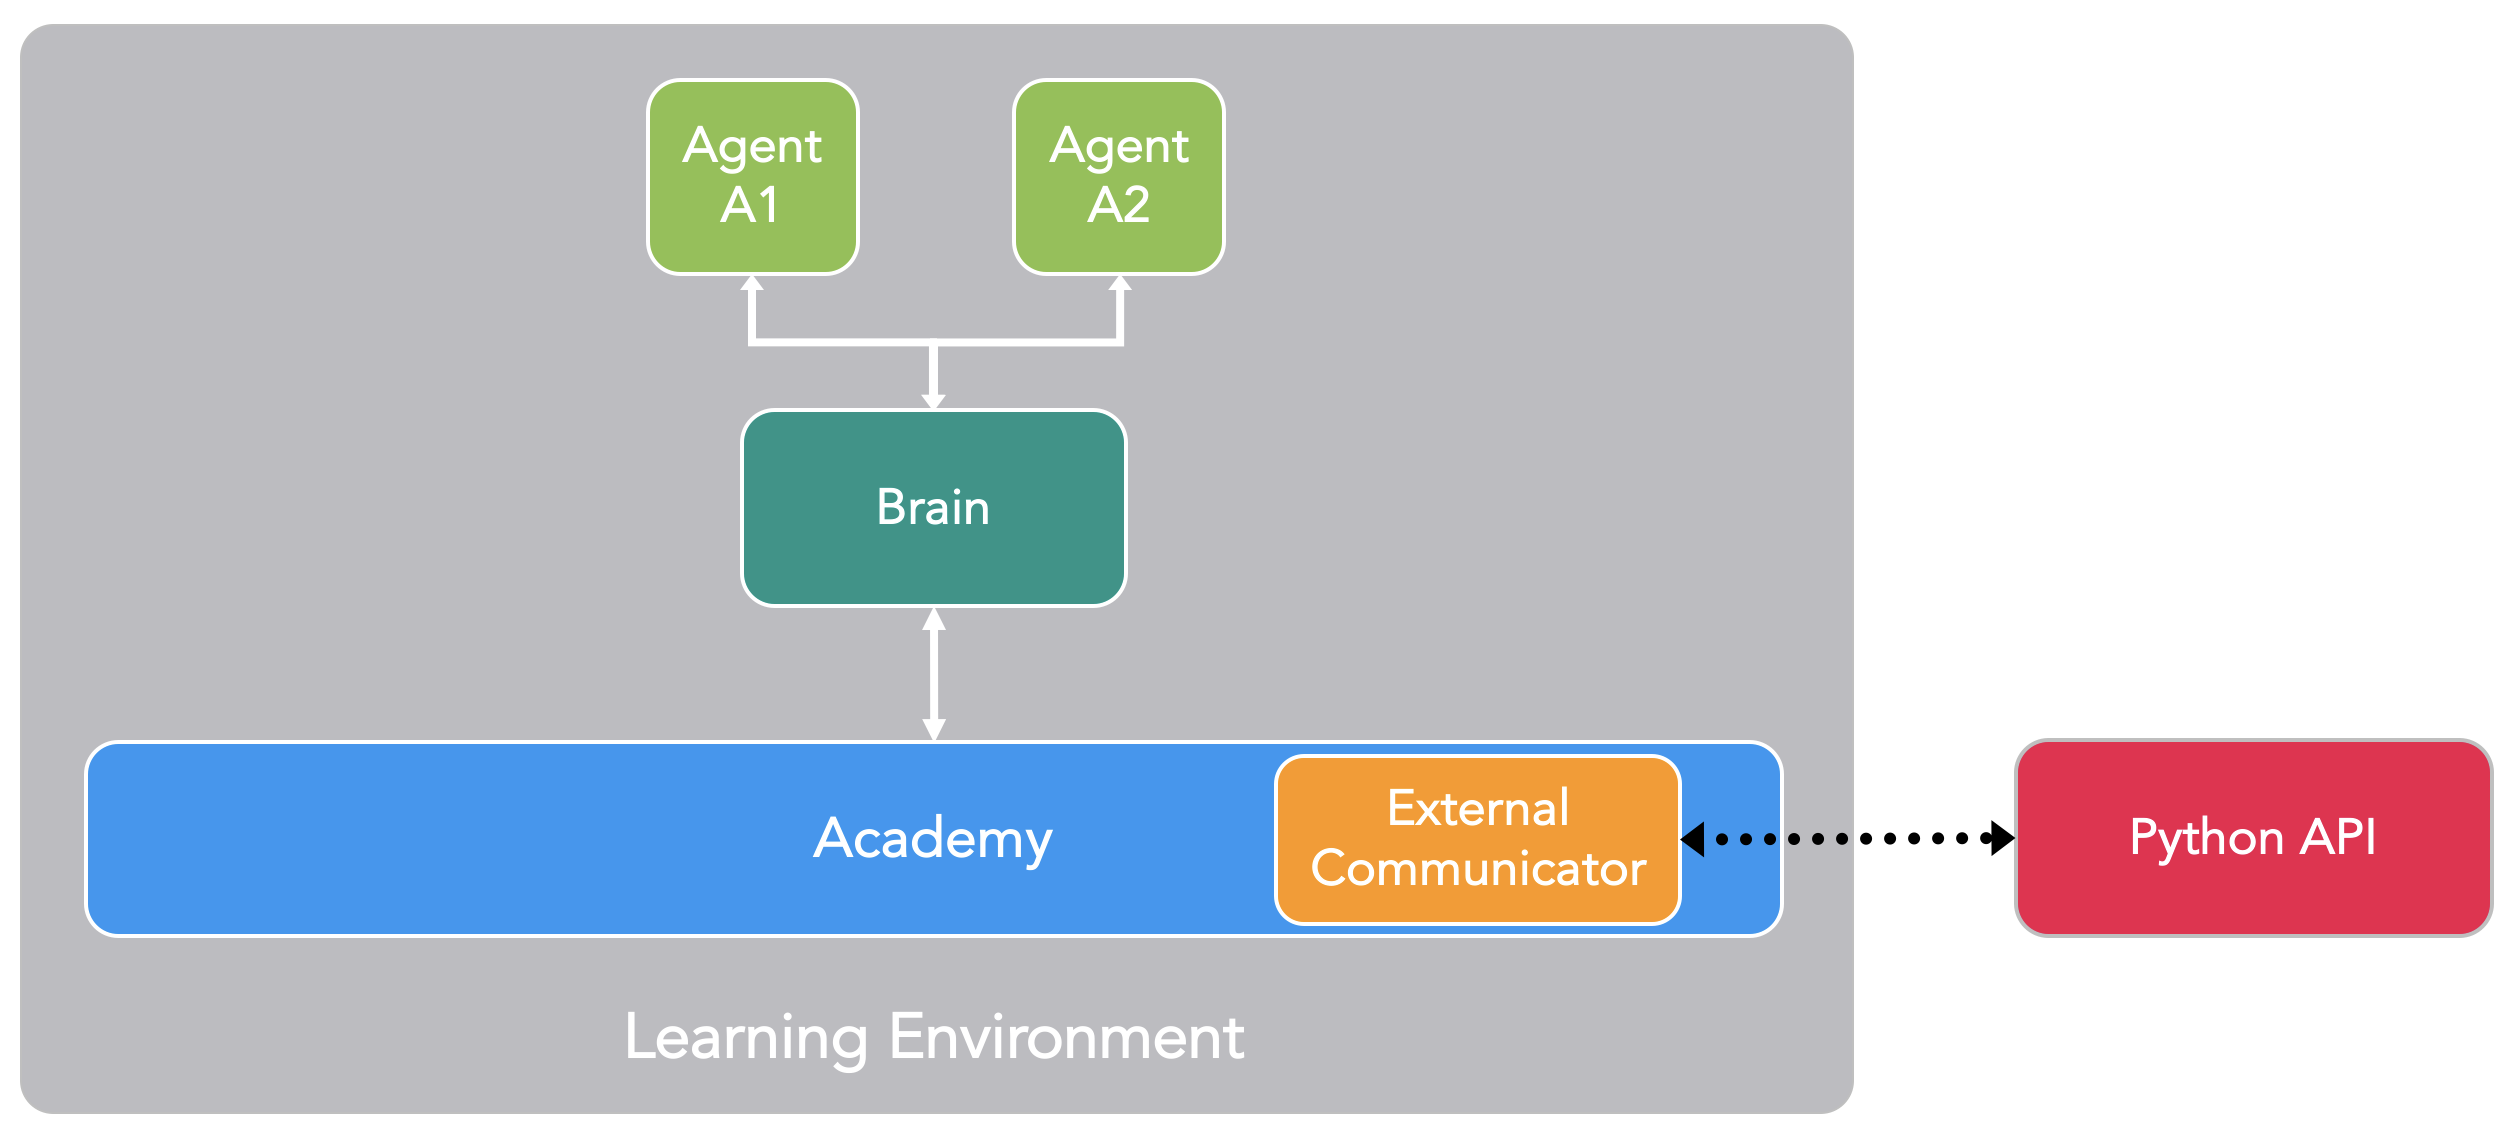
\includegraphics[width=3.5in]{./chapters/imgs/img_unity_mlagents_api_overview.png}
        \caption[unity ml agents overview]{Overview of the Unity ML-Agents architecture. Extracted from \citet{unity-ml-agents}}
        \label{fig:unity-ml-agents-overview}
    \end{figure}

    The previous architecture is exposed to the user through the API, and the basic workflow when using
    this suite is shown in figure 2.9.

    \begin{figure}[!ht]
        \centering
        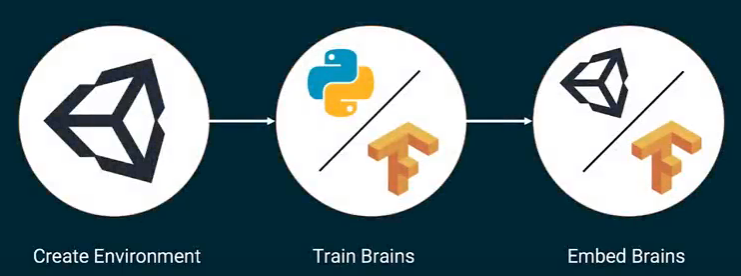
\includegraphics[width=3.5in]{./chapters/imgs/img_unity_mlagents_workflow.png}
        \caption[unity ml agents workflow]{Base workflow used in Unity ML-Agents. Extracted from \citet{unity-ml-agents}}
        \label{fig:unity-ml-agents-workflow}
    \end{figure}